% This is text associated with the open textbook "Open Electromagnetics"
% See immediately below for author, date
% This work is licensed under the Creative Commons Attribution-ShareAlike 4.0 International License. (CC BY-SA 4.0) 
% To view a copy of the license, visit http://creativecommons.org/licenses/by-sa/4.0/

%ORB TITLE Plane Waves at Normal Incidence on a Planar Boundary
%ORB AUTHOR 0        # S.W. Ellingson, Virginia Tech (ellingson@vt.edu)
%ORB DATE 20191116   # yyyymmdd
%ORB ABSTRACT 

\label{m0161_Waves_at_Planar_Boundary} % <-- Must match name of this file and module directory name.  Don't mess with this!

When a plane wave encounters a discontinuity in media, reflection from the discontinuity and transmission into the second medium is possible.
In this section, we consider the scenario illustrated in Figure~\ref{m0161_fPlaneWaveNormalIncidence}:
a uniform plane wave which is normally incident on the planar boundary between two semi-infinite material regions.
By ``normally-incident'' we mean the direction of propagation $\hat{\bf k}$ is perpendicular to the boundary.
We shall assume that the media are ``simple'' and lossless (i.e., the imaginary component of permittivity $\epsilon''$ is equal to zero) and therefore the media are completely defined by a real-valued permittivity and a real-valued permeability.
%
\begin{figure}[b!]
\begin{center}
\pdftooltip{{  % note double braces
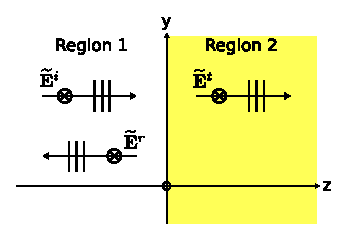
\includegraphics[width=0.8\columnwidth]{modules/m0161_fPlaneWaveNormalIncidence.eps} 
% https://commons.wikimedia.org/wiki/File:Upw_incident_on_planar_boundary.svg
}}{For a z-y coordinate system, plane wave normally incident on a planar boundary. Negative z is region 1 and positive z is region 2. In region 1 capital e tilde superscript i is pointing to the right and capital e tilde superscript r is pointing to the left. In Region 2, capital e tilde superscript t is pointing to the right.}
\end{center}
\centerline{\scriptsize 
\copyright~\hyperref[m0161_fPlaneWaveNormalIncidence_Credit]{C.\ Wang} 
\href{https://creativecommons.org/licenses/by-sa/4.0/}{CC BY-SA 4.0} 
} 
\caption{
\label{m0161_fPlaneWaveNormalIncidence}
A uniform plane wave normally incident on the planar boundary between two semi-infinite material regions.
}
\end{figure}

Figure~\ref{m0161_fPlaneWaveNormalIncidence} shows the wave incident on the boundary, which is located at the $z=0$ plane.
The electric field intensity $\widetilde{\bf E}^i$ of this wave is given by
%
\begin{equation}
\widetilde{\bf E}^i(z) = \hat{\bf x} E_0^i e^{-j\beta_1 z}~\mbox{,}~~z \le 0
\label{m0161_eEi}
\end{equation}
%
where $\beta_1=\omega\sqrt{\mu_1 \epsilon_1}$ is the phase propagation constant in Region~1 and $E_0^i$ is a complex-valued constant. 
$\widetilde{\bf E}^i$ serves as the ``stimulus'' in this problem.
That is, all other contributions to the total field may be expressed in terms of $\widetilde{\bf E}^i$.
In fact, all other contributions to the total field may be expressed in terms of $E_0^i$.

From the plane wave relationships, we determine that the associated magnetic field intensity is
%
\begin{equation}
\widetilde{\bf H}^i(z) = \hat{\bf y} \frac{E_0^i}{\eta_1}  e^{-j\beta_1 z}~\mbox{,}~~z \le 0
\label{m0161_eHi}
\end{equation}
%
where $\eta_1=\sqrt{\mu_1 / \epsilon_1}$ is the wave impedance in Region~1.

The possibility of a reflected plane wave propagating in exactly the opposite direction is inferred from two pieces of evidence:
The general solution to the wave equation, which includes terms corresponding to waves traveling in both $+\hat{\bf z}$ or $-\hat{\bf z}$; and 
the geometrical symmetry of the problem, which precludes waves traveling in any other directions.
The symmetry of the problem also precludes a change of polarization, so the reflected wave should have no $\hat{\bf y}$ component. 
Therefore, we may be confident that the reflected electric field has the form
%
\begin{equation}
\widetilde{\bf E}^r(z) = \hat{\bf x} B e^{+j\beta_1 z}~\mbox{,}~~z \le 0
\label{m0161_eEr}
\end{equation}
%
where $B$ is a complex-valued constant that remains to be determined.  
Since the direction of propagation for the reflected wave is $-\hat{\bf z}$, we have from the plane wave relationships that
%
\begin{equation}
\widetilde{\bf H}^r(z) = -\hat{\bf y} \frac{B}{\eta_1} e^{+j\beta_1 z}~\mbox{,}~~z \le 0
\label{m0161_eHr}
\end{equation}

Similarly, we infer the existence of a ``transmitted'' plane wave propagating on the $z>0$ side of the boundary.  
The symmetry of the problem precludes any direction of propagation other than $+{\bf z}$, and with no possibility of a wave traveling in the $-\hat{\bf z}$ direction for $z>0$. Therefore, we may be confident that the transmitted electric field has the form:
%
\begin{equation}
\widetilde{\bf E}^t(z) = \hat{\bf x} C e^{-j\beta_2 z}~\mbox{,}~~z \ge 0
\label{m0161_eEt}
\end{equation}
%
and an associated magnetic field having the form
%
\begin{equation}
\widetilde{\bf H}^t(z) = \hat{\bf y} \frac{C}{\eta_2} e^{-j\beta_2 z}~\mbox{,}~~z \ge 0
\label{m0161_eHt}
\end{equation}
%
where $\beta_2=\omega\sqrt{\mu_2 \epsilon_2}$ and $\eta_2=\sqrt{\mu_2 / \epsilon_2}$ are the phase propagation constant and wave impedance, respectively, in Region~2.
The constant $C$, like $B$, is a complex-valued constant that remains to be determined.

At this point, the only unknowns in this problem are the complex-valued constants $B$ and $C$.  
Once these values are known, the problem is completely solved.  
These values can be determined by the application of boundary conditions at $z=0$.  
First, recall that the tangential component of the total electric field intensity must be continuous across a material boundary.
To apply this boundary condition, let us define $\widetilde{\bf E}_1$ and $\widetilde{\bf E}_2$ to be the total electric field intensities in Regions~1 and 2, respectively.
The total field in Region~1 is the sum of incident and reflected fields, so
%
\begin{equation}
\widetilde{\bf E}_1(z) = \widetilde{\bf E}^i(z) + \widetilde{\bf E}^r(z)
\end{equation}
%
The field in Region~2 is simply
%
\begin{equation}
\widetilde{\bf E}_2(z) = \widetilde{\bf E}^t(z)
\end{equation}
%
Also, we note that all field components are already tangent to the boundary.
Thus, continuity of the tangential component of the electric field across the boundary requires $\widetilde{\bf E}_1(0)=\widetilde{\bf E}_2(0)$, and therefore
%
\begin{equation}
\widetilde{\bf E}^i(0) + \widetilde{\bf E}^r(0)  = \widetilde{\bf E}^t(0) %~\mbox{, and}
\end{equation}
%
Now employing Equations~\ref{m0161_eEi}, \ref{m0161_eEr}, and \ref{m0161_eEt}, we obtain:
%
\begin{equation}
E_0^i + B = C
\label{m0161_eBCE}
\end{equation}

Clearly a second equation is required to determine both $B$ and $C$.
This equation can be obtained by enforcing the boundary condition on the magnetic field.  
Recall that any discontinuity in the tangential component of the total magnetic field intensity must be supported by a current flowing on the surface.
There is no impressed current in this problem, and there is no reason to suspect a current will arise in response to the fields present in the problem.
Therefore, the tangential components of the magnetic field must be continuous across the boundary.
This becomes the same boundary condition that we applied to the total electric field intensity, so the remaining steps are the same.
We define $\widetilde{\bf H}_1$ and $\widetilde{\bf H}_2$ to be the total magnetic field intensities in Regions~1 and 2, respectively.
The total field in Region~1 is
%
\begin{equation}
\widetilde{\bf H}_1(z) = \widetilde{\bf H}^i(z) + \widetilde{\bf H}^r(z)
\end{equation}
%
The field in Region~2 is simply
%
\begin{equation}
\widetilde{\bf H}_2(z) = \widetilde{\bf H}^t(z)
\end{equation}
%
The boundary condition requires $\widetilde{\bf H}_1(0)=\widetilde{\bf H}_2(0)$, and therefore
%
\begin{equation}
\widetilde{\bf H}^i(0) + \widetilde{\bf H}^r(0)  = \widetilde{\bf H}^t(0) %~\mbox{, and}
\end{equation}
%
Now employing Equations~\ref{m0161_eHi}, \ref{m0161_eHr}, and \ref{m0161_eHt}, we obtain:
%
\begin{equation}
\frac{E_0^i}{\eta_1} - \frac{B}{\eta_1} = \frac{C}{\eta_2}
\label{m0161_eBCH}
\end{equation}

Equations~\ref{m0161_eBCE} and \ref{m0161_eBCH} constitute a linear system of two simultaneous equations with two unknowns.  
A straightforward method of solution is to first eliminate $C$ by substituting the left side of Equation~\ref{m0161_eBCE} into Equation~\ref{m0161_eBCH}, and then to solve for $B$.   One obtains:
%
\begin{equation}
B = \Gamma_{12} E_0^i
\label{m0161_eB}
\end{equation}
%
where
%
\begin{equation}
\boxed{
\Gamma_{12}  \triangleq \frac{\eta_2-\eta_1}{\eta_2+\eta_1} 
}
\label{m0161_eG}
\end{equation}
%
$\Gamma_{12}$ is known as a {\it reflection coefficient}.  
\index{reflection coefficient}
The subscript ``12'' indicates that this coefficient applies for incidence from Region~1 toward Region~2. 
We may now solve for $C$ by substituting Equation~\ref{m0161_eB} into Equation~\ref{m0161_eBCE}.  We find:
%
\begin{equation}
C = (1+\Gamma_{12})~E_0^i
\end{equation}
%
Now summarizing the solution:
%
\begin{equation}
\boxed{ \widetilde{\bf E}^r(z) = \hat{\bf x} \Gamma_{12} E_0^i e^{+j\beta_1 z} ~~~\mbox{,}~~z \le 0 } 
\label{m0161_eErf}
\end{equation}
%
\begin{equation}
\boxed{ \widetilde{\bf E}^t(z) = \hat{\bf x} \left( 1+\Gamma_{12} \right) E_0^i e^{-j\beta_2 z} ~~~\mbox{,}~~z \ge 0 }
\label{m0161_eEtf}
\end{equation}
%
%%%%%%%%%%%%%%%%%%%%%%%%%%%%%%%%%%%%%%%%%%%%%%%
%ORB HIGHLIGHT
\begin{mdframed}[backgroundcolor=yellow!20,nobreak=true] 
Equations~\ref{m0161_eErf} and \ref{m0161_eEtf} are the reflected and transmitted fields, respectively, in response to the incident field given in Equation~\ref{m0161_eEi} in the normal incidence scenario shown in Figure~\ref{m0161_fPlaneWaveNormalIncidence}.
\end{mdframed}
%%%%%%%%%%%%%%%%%%%%%%%%%%%%%%%%%%%%%%%%%%%%%%%
%
Expressions for $\widetilde{\bf H}^r$ and $\widetilde{\bf H}^t$ may be obtained by applying the plane wave relationships to the preceding expressions.

It is useful to check this solution by examining some special cases.
First: If the material in Region~2 is identical to the material in Region~1, then there should be no reflection and $\widetilde{\bf E}^t=\widetilde{\bf E}^i$.
In this case, $\eta_2=\eta_1$, so $\Gamma_{12}=0$, and we obtain the expected result.

A second case of practical interest is when Region~2 is a perfect conductor.
\index{conductor!perfect}
First, note that this may seem at first glance to be a violation of the ``lossless'' assumption made at the beginning of this section.
While it is true that we did not explicitly account for the possibility of a perfect conductor in Region~2, let's see what the present analysis has to say about this case.
If the material in Region~2 is a perfect conductor, then there should be no transmission since the electric field is zero in a perfect conductor.
In this case, $\eta_2=0$ since the ratio of electric field intensity to magnetic field intensity is zero in Region~2, and subsequently $\Gamma_{12}=-1$ and $1+\Gamma_{12}=0$.  
As expected, $\widetilde{\bf E}^t$ is found to be zero, and the reflected electric field experiences a sign change as required to enforce the boundary condition $\widetilde{\bf E}^i(0)+\widetilde{\bf E}^r(0)=0$. 
Thus, we obtained the correct answer because we were able to independently determine that $\eta_2=0$ in a perfect conductor.
%
%%%%%%%%%%%%%%%%%%%%%%%%%%%%%%%%%%%%%%%%%%%%%%%
%ORB HIGHLIGHT
\begin{mdframed}[backgroundcolor=yellow!20,nobreak=true] 
When Region~2 is a perfect conductor, the reflection coefficient $\Gamma_{12}=-1$ and the solution described in Equations~\ref{m0161_eErf} and \ref{m0161_eEtf} applies. 
\end{mdframed}
%%%%%%%%%%%%%%%%%%%%%%%%%%%%%%%%%%%%%%%%%%%%%%%

It may be helpful to note the very strong analogy 
\index{transmission line!analogy for wave propagation}
between reflection of the electric field component of a plane wave from a planar boundary and the reflection of a voltage wave in a transmission line from a terminating impedance.  
In a transmission line, the voltage reflection coefficient $\Gamma$ is given by 
%
\begin{equation}
\Gamma = \frac{Z_L-Z_0}{Z_L+Z_0}
\end{equation} 
%
where $Z_L$ is the load impedance and $Z_0$ is the characteristic impedance of the transmission line.
Comparing this to Equation~\ref{m0161_eG}, we see $\eta_1$ is analogous to $Z_0$ and $\eta_2$ is analogous to $Z_L$.
Furthermore, we see the special case $\eta_2=\eta_1$, considered previously, is analogous to a matched load, and
the special case $\eta_2=0$, also considered previously, is analogous to a short-circuit load.

In the case of transmission lines, we were concerned about what fraction of the power was delivered into a load and what fraction of the power was reflected from a load.
A similar question applies in the case of plane wave reflection.
In this case, we are concerned about what fraction of the power \emph{density} is transmitted into Region~2 and what fraction of the power \emph{density} is reflected from the boundary.
The time-average power density $S_{ave}^i$ associated with the incident wave is:
%
\begin{equation}
S_{ave}^i = \frac{|E^i_0|^2}{2\eta_1} 
\end{equation}
%
presuming that $E^i_0$ is expressed in peak (as opposed to rms) units.
Similarly, the time-average power density $S_{ave}^r$ associated with the reflected wave is:
%
\begin{flalign}
S_{ave}^r &= \frac{\left|\Gamma_{12} E_0^i\right|^2}{2\eta_1} \nonumber \\
          &= \left|\Gamma_{12}\right|^2 \frac{\left|E_0^i\right|^2}{2\eta_1} \nonumber \\
          &= \left|\Gamma_{12}\right|^2 S_{ave}^i \label{m0161_eSaver}
\end{flalign}
%  
From the principle of conservation of power, the power density $S_{ave}^t$ transmitted into Region~2 must be equal to the incident power density minus the reflected power density.
Thus:
%
\begin{flalign}
S_{ave}^t &= S_{ave}^i - S_{ave}^r \nonumber \\
          &= \left( 1-|\Gamma_{12}|^2 \right)S_{ave}^i
\end{flalign}
%
In other words, the ratio of power density transmitted into Region~2 to power density incident from Region~1 is
%
\begin{equation}
\boxed{ \frac{S_{ave}^t}{S_{ave}^i} = 1-|\Gamma_{12}|^2 } 
\label{m0161_eSavet}
\end{equation}
%
Again, the analogy to transmission line theory is evident.
%
%%%%%%%%%%%%%%%%%%%%%%%%%%%%%%%%%%%%%%%%%%%%%%%
%ORB HIGHLIGHT
\begin{mdframed}[backgroundcolor=yellow!20,nobreak=true] 
The fractions of power density reflected and transmitted relative to power density incident are given in terms of the reflection coefficient $\Gamma_{12}$ by Equations~\ref{m0161_eSaver} and \ref{m0161_eSavet}, respectively. 
\end{mdframed}
%%%%%%%%%%%%%%%%%%%%%%%%%%%%%%%%%%%%%%%%%%%%%%%
  
Finally, note that a variety of alternative expressions exist for the reflection coefficient $\Gamma_{12}$.
Since the wave impedance $\eta=\sqrt{\mu/\epsilon}$ in lossless media, and since most lossless materials are non-magnetic (i.e., exhibit $\mu\approx\mu_0$), it is possible to express $\Gamma_{12}$ purely in terms of permittivity for these media.
Assuming $\mu=\mu_0$, we find:
%
\begin{flalign}
\Gamma_{12} &= \frac{\eta_2-\eta_1}{\eta_2+\eta_1} \nonumber \\
            &= \frac{\sqrt{\mu_0/\epsilon_2}-\sqrt{\mu_0/\epsilon_1}}{\sqrt{\mu_0/\epsilon_2}+\sqrt{\mu_0/\epsilon_1}} \nonumber \\
            &= \frac{\sqrt{\epsilon_1}-\sqrt{\epsilon_2}}{\sqrt{\epsilon_1}+\sqrt{\epsilon_2}}  
\end{flalign}
%
Moreover, recall that permittivity can be expressed in terms of relative permittivity; that is, $\epsilon=\epsilon_r\epsilon_0$. 
Making the substitution above and eliminating all extraneous factors of $\epsilon_0$, we find:
%
\begin{equation}
\Gamma_{12} = \frac{\sqrt{\epsilon_{r1}}-\sqrt{\epsilon_{r2}}}{\sqrt{\epsilon_{r1}}+\sqrt{\epsilon_{r2}}}
\label{m0161_eGer}
\end{equation}
%
where $\epsilon_{r1}$ and $\epsilon_{r2}$ are the relative permittivities in Regions~1 and 2, respectively.

%%%%%%%%%%%%%%%%%%%%%%%%%%%%%%%%%%%%%%%%%%%%%%%
%ORB EXAMPLE
~\\ \begin{example} 
\begin{mdframed}[backgroundcolor=brown!20,linecolor=brown!20]\raggedright
Radio reflection from the surface of the Moon.
\\~\\
At radio frequencies, the Moon can be modeled as a low-loss dielectric with relative permittivity of about 3.
Characterize the efficiency of reflection of a radio wave from the Moon.\\
~\\

\noindent
{\bf Solution}. At radio frequencies, a wavelength is many orders of magnitude less than the diameter of the Moon, so we are justified in treating the Moon's surface as a planar boundary between free space and a semi-infinite region of lossy dielectric material.
The reflection coefficient is given approximately by Equation~\ref{m0161_eGer} with $\epsilon_{r1}\approx 1$ and $\epsilon_{r2}\sim 3$.
Thus, $\Gamma_{12}\sim-0.27$.
Subsequently, the fraction of power reflected from the Moon relative to power incident is $\left|\Gamma_{12}\right|^2\sim 0.07$; i.e., about 7\%.
\end{mdframed}
% note figures will need to go between "\end{mdframed}" and "\end{example}"
\end{example}
%%%%%%%%%%%%%%%%%%%%%%%%%%%%%%%%%%%%%%%%%%%%%%%

In optics, it is common to make the definition $n\triangleq \sqrt{\epsilon_r}$ where $n$ is known as the \emph{index of refraction} 
\index{index of refraction}
or \emph{refractive index}.\footnote{A bit of a misnomer, since the definition applies even when there is no refraction, as in the scenario considered in this section.}
In terms of the indices of refraction $n_1$ and $n_2$ for Regions~1 and 2, respectively:
%
\begin{equation}
\Gamma_{12} = \frac{n_1-n_2}{n_1+n_2}
\end{equation}

%%%%%%%%%%%%%%%%%%%%%

{\bf Additional Reading:}
\begin{itemize}
\item ``\href{https://en.wikipedia.org/wiki/Refractive_index}{Refractive index}'' on Wikipedia.
\end{itemize}



